\documentclass[11pt,a4paper]{article}

\usepackage[utf8]{inputenc}
\usepackage[T1]{fontenc}
\usepackage[english]{babel}
\usepackage[a4paper,margin=2.4cm]{geometry}

\usepackage{amsmath, amssymb, amsthm}
\usepackage{mathtools}
\usepackage{booktabs}
\usepackage{tabularx}
\usepackage{array}
\usepackage{caption}
\usepackage{float}
\usepackage{enumitem}
\usepackage{microtype}
\usepackage{xcolor}
\usepackage{listings}
\usepackage{fancyhdr}
\usepackage{titlesec}
\usepackage{graphicx}
\usepackage[hidelinks]{hyperref}

%  ---  Palette shared with the companion reports  ---
\definecolor{ink}{RGB}{26,30,36}
\definecolor{slate}{RGB}{92,101,112}
\definecolor{mist}{RGB}{233,235,238}
\definecolor{rulegrey}{RGB}{188,194,201}
\definecolor{steel}{RGB}{47,72,102}
\definecolor{signal}{RGB}{160,32,45}

\hypersetup{
    colorlinks=true,
    linkcolor=steel,
    citecolor=steel,
    urlcolor=steel,
    pdftitle={When Planning Pays},
    pdfauthor={Haniel Ulises},
}

\color{ink}

\setlength{\headheight}{22pt}
\pagestyle{fancy}
\fancyhf{}
\fancyhead[L]{\small\textcolor{slate}{\itshape When Planning Pays}}
\fancyhead[R]{\small\textcolor{slate}{\thepage}}
\renewcommand{\headrulewidth}{0.4pt}
\renewcommand{\headrule}{\hbox to\headwidth{\color{rulegrey}\leaders\hrule height \headrulewidth\hfill}}

\titleformat{\section}{\normalfont\large\bfseries\color{ink}}{\thesection}{0.7em}{}
\titleformat{\subsection}{\normalfont\normalsize\bfseries\color{ink}}{\thesubsection}{0.7em}{}
\titleformat{\paragraph}[runin]{\normalfont\bfseries\color{slate}}{}{0em}{}[.]

\captionsetup{font=small, labelfont={bf,color=slate}, textfont=footnotesize}

\theoremstyle{definition}
\newtheorem{definition}{Definition}
\newtheorem{proposition}{Proposition}
\newtheorem{lemma}{Lemma}
\newtheorem{corollary}{Corollary}
\newtheorem{remark}{Remark}

\lstdefinestyle{sys}{
    backgroundcolor=\color{mist},
    basicstyle=\ttfamily\scriptsize\color{ink},
    keywordstyle=\color{steel}\bfseries,
    commentstyle=\color{slate}\itshape,
    morecomment=[l]{;},
    morekeywords={:action,:precondition,:effects,:action-type,:observability-conditions,:goal,:parameters},
    frame=single,
    rulecolor=\color{rulegrey},
    framesep=5pt,
    xleftmargin=6pt,
    breaklines=true,
    showstringspaces=false,
    columns=fullflexible,
}
\lstset{style=sys}

\newcommand{\Bop}[1]{B_{#1}}
\newcommand{\code}[1]{\texttt{\small #1}}
\newcommand{\blocked}{\mathit{blocked}}
\newcommand{\delivered}{\mathit{delivered}}
\newcommand{\merged}{\mu}

\begin{document}

\begin{titlepage}
\centering
\vspace*{2.4cm}
{\color{rulegrey}\rule{\textwidth}{0.8pt}}\\[0.9cm]
{\LARGE\bfseries When Planning Pays\par}
\vspace{0.5cm}
{\large\color{slate} Epistemic Planning Against Map-Sharing Protocols:\\
the Conditions Under Which Sharing Is Enough, and What Happens Without Each\par}
\vspace{0.7cm}
{\color{rulegrey}\rule{\textwidth}{0.8pt}}\\[1.4cm]

{\large Haniel Ulises\par}
\vspace{0.3cm}
{\color{slate} Epistemic Robotics}\\
\vspace{0.15cm}
{\color{slate}\today}

\vfill
{\color{slate}\small
A fleet whose maps have gone stale can be repaired by a plan that decides who
tells whom what, or by a protocol that shares maps without deciding anything:
flooding every reading, asking before going, or gossiping. This report asks when
the plan is worth its cost, and why. We prove that flooding with a merge rule
that orders readings as they were taken leaves every robot holding the fleet's
freshest reading of every bay, so that with an unlimited budget on a connected
radio graph, goals that mention only the floor, and clocks that agree, a hauler
acting on its flooded map does what it would do knowing everything the fleet
saw. The plan then has nothing to add. Each condition, removed, separates the two,
and for each we state the separation and measure it on 2400 instances drawn
under four regimes, every strategy run on the same instances. Under a message
budget the plan reached 95\% success with 3 to 6 messages, flooding with 96 to
512. With a contractor robot that must not learn of a change, flooding kept the
secret in exactly the instances in which no robot saw the change, 4.5\% of
eight-robot shifts, and pulling did as badly once the contractor hauled; the plan succeeded on
all of them. When the open bay was seen by nobody and known only by elimination,
the plan sent a median of one or two messages, against 224 to 336 for flooding.
Clock skew broke recency, and not sharing: a merge by the schedule's version
matched the plan at every deviation. In Gazebo, eight robots on one floor with a
contractor ran four strategies; each did what the analysis says, and only the plan
delivered every hauler without telling the contractor.}
\vspace{1.2cm}
\end{titlepage}

\tableofcontents
\newpage

%  ======================================================================
\section{Scope}
\label{sec:scope}

The stale-maps report~\cite{ulises2026sm} showed a plan that repairs a fleet's
stale maps with three messages, where sharing every map took 168. That comparison
leaves two questions open. Is the plan's advantage a matter of degree, a smaller
message count, which a protocol with a sensible merge rule approaches by sending
more? And if there are tasks a sharing protocol cannot do at any message count,
which ones, and what property of them is responsible? A comparison that only
shows the plan winning on its own floor answers neither.

This report answers both by separating them. Section~\ref{sec:enough} proves a
proposition stating four conditions under which flooding does whatever any
strategy can, so that an epistemic planner has nothing to offer but a smaller
count. Section~\ref{sec:separations} removes the conditions one at a time and
states, for each, what goes wrong for the protocols and what the plan does
instead. Section~\ref{sec:study} measures every separation on instances drawn
for the purpose, paired so that each comparison is between strategies on the same
instance. Section~\ref{sec:floor} runs one of them on the floor in Gazebo.

Five claims are advanced.

\begin{enumerate}[leftmargin=1.4em, itemsep=2pt]
  \item With an unlimited budget on a connected graph, a merge order consistent
        with the order of the readings, and goals over the floor alone, flooding
        leaves every robot with the fleet's freshest map, and its haulers do what
        they would do knowing every reading in the fleet
        (Proposition~\ref{prop:enough}).
  \item Under a budget, flooding spends at least $2|E||T|$ messages before every
        robot has heard every neighbour once, independent of need, where a
        strategy that knows who needs what can succeed with one message per
        misled hauler (Proposition~\ref{prop:budget}). Pulling is limited to
        one hop (Corollary~\ref{cor:pull}).
  \item Under a goal that a robot must not believe a fact, flooding succeeds
        exactly when no robot observed it (Proposition~\ref{prop:secret}); the
        study agrees on 600 of 600 instances.
  \item When a bay is known only by elimination, a protocol of readings needs up
        to $B-1$ messages where one report of a belief suffices
        (Proposition~\ref{prop:elim}).
  \item Clock skew inverts two readings when the offset between their clocks
        exceeds the time between them (Proposition~\ref{prop:skew}); the
        remedy is a merge by version, which needs no planner.
\end{enumerate}

The conclusion is in two parts. The plan outperforms sharing when messages are
scarce, when the goal is about what some robot believes or must not believe, and
when what a robot needs to be told is an inference of the sender's and not an
observation. It does not outperform flooding with a sound merge rule under an
unlimited budget and first-order goals, and the advantage it shows under clock
skew belongs to the version order, not to planning.

%  ======================================================================
\section{The setting}
\label{sec:setting}

\paragraph{Instances} A fleet of robots $A$, $|A| = n$, shares a floor with bays
$T$, $|T| = B$. A radio graph $G = (A, E)$ says which pairs can exchange messages;
in some instances every pair is linked. A forklift changes some bays during the
shift; each change is seen by a random subset of the robots, each robot with
probability $0.3$. Some robots haul: after the messages, a hauler crosses a bay
it believes open, and the shift succeeds when every crossing is through an open
bay. A regime adds to this: a message budget, a set of contractor robots that
must not learn a change, pairs of haulers that must cross together, a bay known
only by elimination, or clocks that disagree.

\paragraph{Readings} Each robot holds, for each bay, a reading
$\rho_i(t) = (v, s, k, o)$: a value $v$, open or blocked,
the stamp $s$ at which it was taken on its observer's clock, the version $k$ of the
bay it reflects (the number of the forklift's slot it saw, $0$ for the shift
map), and the observer $o$. Observation is transient: a robot reads a change as it
happens and does not read the bay again.

\paragraph{Messages} A message is one robot's reading of one bay sent to a robot
it is linked to, the unit in which the plan's map reports are counted. On receipt,
$\rho_j(t) \leftarrow \mathrm{merge}(\rho_j(t), \rho_i(t))$, where the merge rule
is one of
\emph{recency}, the reading with the larger stamp;
\emph{version}, the reading with the larger version, the forklift's schedule used
as a logical clock~\cite{lamport1978};
\emph{overwrite}, the sender's; or
\emph{confidence}, the receiver's, which is what \code{epistemic\_slam::fuse} does
with readings of $0$ and $100$~\cite{ulises2026sm}.

\paragraph{Protocols}
\begin{itemize}[leftmargin=1.4em, itemsep=2pt]
  \item \emph{Flood}: every robot sends every neighbour its reading of every
        bay, then re-sends a bay to a neighbour only when its reading has changed
        since it last sent it there, round after round until nothing changes.
  \item \emph{Pull}: each hauler asks every neighbour about every bay; a request
        and its reply are two messages. There are no relays.
  \item \emph{Gossip}: random linked pairs exchange whole maps, until twenty
        exchanges in a row change nothing.
\end{itemize}
A budget caps the messages; a protocol stops when it is spent. Every hauler then
chooses, among the bays its map shows open, the one with the freshest reading under
its merge order. In the elimination regime a hauler may also conclude that a bay
is open from readings of every other bay as blocked.

\paragraph{The plan} The instance is an epistemic planning
task~\cite{ba2011}, written in EPDDL~\cite{ulises2026sm} and updated by the
product update~\cite{bms1998}: a
change is an action whose observers see it \emph{Fully} and the rest
\emph{Obliviously}; a map report \code{send-open(i,j,t)} or
\code{send-blocked(i,j,t)} has the sender \emph{Fully}, the receiver as
\emph{Recipient}, and every other robot \emph{Oblivious}, and requires that the
sender believe the receiver believes the opposite; a crossing requires the hauler
to believe the bay open and the bay to be open.

\begin{lstlisting}[language={}]
(:action send-open :parameters (?i ?j - agent ?t - bay)
  :action-type (map-report (e-says-open ?i ?j ?t) (e-opened ?t) (nil))
  :precondition (and (radio) (settled) (link ?i ?j)
                     ([?i] (not (blocked ?t))) ([?i] ([?j] (blocked ?t))))
  :observability-conditions (:and (?i Fully) (?j Recipient) (default Oblivious)))
\end{lstlisting}

The task is grounded by \code{plank} and solved by Aletheia with consistent
beliefs required, as ePlanSys solves it on the floor. The planner's search does not
minimise messages, so the policy is shortened by action elimination: each message,
latest first, is dropped if every action stays applicable and the goal is still
reached. This removed 6179 messages from 1112 of the 2390 policies found. Each
policy's messages are then replayed on the readings, and a policy that succeeds in
the model must succeed there; the study stops if one does not, and none did.

%  ======================================================================
\section{When sharing is enough}
\label{sec:enough}

For a bay $t$ and a merge order $\preceq$, let $\merged(t)$ be the
$\preceq$-greatest reading of $t$ held by any robot, and $\merged$ the map that has
it for every bay: the fleet's freshest map.

\begin{proposition}[Flooding computes the freshest map]
\label{prop:enough}
Let $G$ be connected, the budget unlimited, and the merge rule recency or version.
Flooding stops with $\rho_i = \merged$ for every robot $i$, after at least
$2|E|B$ and at most $2|E|\sum_t c_t$ messages, where $c_t$ is the number of
distinct readings of bay $t$ in the fleet.
\end{proposition}

\begin{proof}
For one bay, both merges keep the $\preceq$-greater of two readings, and taking the
greater is associative, commutative and idempotent, so the reading a robot ends
with is the greatest among those that reach it, in any order. Let $i^*$ hold
$\merged(t)$. By induction on $d$, after $d$ rounds every robot at distance $d$
from $i^*$ holds it: a neighbour of such a robot is sent its reading in the next
round, since the reading changed when it was received or is the one first sent.
$G$ being connected, every robot holds $\merged(t)$ after at most the graph's
diameter rounds, and a reading never decreases, so it keeps it. In the first round
each robot sends each neighbour each bay, $2|E|B$ messages. Afterwards $i$ sends
$j$ bay $t$ again only when $\rho_i(t)$ has changed, which happens at most
$c_t - 1$ times, since each change is to a greater reading among the $c_t$.
\end{proof}

\begin{corollary}[When the plan has nothing to add]
\label{cor:enough}
Suppose further that the goal mentions only the floor (every hauler crosses an
open bay) and that the merge order is consistent with the order in which readings
were taken. Then every hauler crosses the bay it would choose holding every
reading in the fleet. In particular, if $\merged$ shows some open bay whose
reading is fresher than every reading showing a blocked bay open, flooding
succeeds.
\end{corollary}

\begin{proof}
A hauler's choice depends on its map alone, which is $\merged$ by
Proposition~\ref{prop:enough}. When the order is consistent with time, the
freshest reading of a bay is the latest observation of it, the best any strategy
built on the robots' observations can give a hauler. The freshest open reading
is then of an open bay by the hypothesis, and the hauler chooses it.
\end{proof}

The four conditions are an unlimited budget, a connected graph, a goal over the
floor alone, and a merge order consistent with time. The study's budget instances
meet all four when the budget is unlimited, and there flooding succeeded on 800 of
800, as did the plan. With every condition met, what the plan saves is messages.
Each condition, removed, makes a difference of another kind.

%  ======================================================================
\section{Removing each condition}
\label{sec:separations}

\subsection{A budget}

\begin{proposition}[Flooding pays before it knows]
\label{prop:budget}
Flooding sends $2|E|B$ messages in its first round whatever the instance, and
which robot hears which reading within a budget $b < 2|E|B$ depends on the order of
sending, not on which haulers are misled. A strategy that knows who needs what can
succeed with as few messages as the haulers misled by their own maps, each sent one
reading along a path from a robot holding it, and needs at least one per misled
hauler.
\end{proposition}

\begin{proof}
The first claim is the first round of Proposition~\ref{prop:enough}. A hauler whose
map leads it into a blocked bay, or to no bay, must receive at least one reading
before it crosses, which is the lower bound. A reading sent along a shortest path
from a robot that holds it reaches the hauler in as many messages as the path is
long; on a complete graph that is one.
\end{proof}

For eight robots and three bays on a complete graph, $2|E|B = 168$; flooding's
measured median was 189. For sixteen it is 720, against a measured 765. The plan
sent a median of 2 and 4. The plan can find the short sends because its
preconditions, $\Bop{i}\neg\blocked(t) \wedge \Bop{i}\Bop{j}\blocked(t)$, single out
the pairs in which the sender holds a reading the receiver lacks.

\begin{corollary}[Pull is one hop]
\label{cor:pull}
A hauler that pulls ends with the freshest reading among its own and its
neighbours'. On a radio graph pull succeeds only if every misled hauler has a
neighbour holding a reading that steers it right.
\end{corollary}

On sparse radio graphs pull succeeded on 58\% and 66\% of shifts at any budget.
It failed when no neighbour of a misled hauler had seen the clearing: in 105 shifts
a hauler then believed no bay open, and in 49 it had heard of neither change and
drove into the staged bay.

\subsection{A goal over beliefs}

\begin{proposition}[Flooding keeps a secret only if nobody knew it]
\label{prop:secret}
Let a contractor $c$ be connected to the robots that observed a change of bay $t$
to blocked, and let the goal require $\neg\Bop{c}\blocked(t)$. With an unlimited
budget and a merge consistent with time, flooding meets the goal if and only if no
robot observed the change.
\end{proposition}

\begin{proof}
If some robot observed it, its reading is the freshest of $t$, so
$\rho_c(t) = \merged(t)$ shows $t$ blocked by Proposition~\ref{prop:enough}. If none
did, every reading of $t$ in the fleet is the shift map's, which shows $t$ open.
\end{proof}

The prediction is exact on the study's instances: flooding succeeded on 9, 2 and
10 of the 200 instances of each secrecy cell, in each case precisely the instances
in which nobody saw the staging. Pull sends only to haulers and keeps the secret
when no contractor hauls (100\%), but a contractor that hauls asks every neighbour
about every bay and learns it in the same instances as flooding (5\%). The plan
succeeded on all 600. It can, because a map report is \emph{Recipient}-observable:
only sender and receiver learn from it, and the goal's
$\neg\Bop{c}\blocked(t)$ is a constraint the search satisfies by sending $c$ nothing
about $t$. No protocol whose sends do not depend on the receiver's goals can do
this, and adding such a dependency is writing the plan by hand.

\begin{remark}[Joint crossing is not a separation without a budget]
A pair of haulers must cross the same bay, each believing it open and believing
the other does: $\Bop{h}\Bop{k}\neg\blocked(t)$ and its converse. Under the
conditions of Proposition~\ref{prop:enough}, every robot holds $\merged$ and uses the
same choice rule, so the pair agree without either believing anything of the
other; the second-order belief is replaced by a common protocol. The study agrees:
every protocol succeeded on all 400 joint instances without a budget. Under a
budget the maps differ and the pair can split, and the plan reached 95\% at 4
messages where no protocol did at 64.
\end{remark}

\subsection{Knowledge that is not an observation}

In the elimination regime exactly one of $B$ bays is open, which every robot
knows, and which one is not. Each robot sees each bay with probability 0.3, and
the open bay may be seen by nobody; the fleet's distributed
knowledge~\cite{fhmv1995} determines it. The model is S5.

\begin{proposition}[A conclusion is cheaper than its premises]
\label{prop:elim}
A hauler that holds readings of $m$ of the $B - 1$ blocked bays and none of the
open one needs, under a protocol of readings, at least $B - 1 - m$ further
messages, or one reading of the open bay if any robot has one. A report of a
belief, $\code{tell-open}(i, h, t)$, from a robot that knows $t$ open by
elimination, needs one.
\end{proposition}

\begin{proof}
A reading carries what its observer saw. Without a reading of $t$ the hauler can
conclude $t$ open only when every other bay is read blocked. The report is a private
announcement of $\Bop{i}\mathit{open}(t)$, which, beliefs being knowledge in S5,
gives the hauler $\mathit{open}(t)$ in one message.
\end{proof}

The plan sent a median of 2 messages with four bays and 1 with six; flooding sent
224 and 336, pull 112 and 168. Flooding without the hauler's inference by
elimination failed on 8 of the 200 instances of each cell at any budget, those in
which no robot saw the open bay. Here the plan's advantage is the content of a message: a report of a
belief carries the sender's inference, a reading only an observation.

\subsection{Clocks that disagree}

\begin{proposition}[Recency inverts readings]
\label{prop:skew}
Let two readings of a bay be taken at true times $\tau < \tau'$ by robots whose
clocks are off by $o$ and $o'$. Recency prefers the earlier one if and only if
$o - o' > \tau' - \tau$. For offsets drawn independently from
$\mathcal{N}(0, \sigma^2)$ this has probability
$\Phi\bigl(-(\tau' - \tau)/(\sigma\sqrt{2})\bigr)$. The version order is consistent
with time whatever the clocks.
\end{proposition}

\begin{proof}
The stamps are $\tau + o$ and $\tau' + o'$; the first is greater exactly when
$o - o' > \tau' - \tau$. The difference of two independent normal offsets is normal
with variance $2\sigma^2$. Versions are the forklift's slot numbers, which increase
with the schedule and do not depend on any clock.
\end{proof}

In the skew instances one bay is cleared and staged again ten seconds later, and
each robot's shift map, stamped at its own clock's zero, is fifteen seconds older
than the clearing of another. At $\sigma = 10$\,s some bay's readings were inverted
in 63 of 200 instances, and every recency protocol failed on 46 of them; at
$\sigma = 40$\,s, 128 and 111. Under recency, every robot ending with
$\merged$ predicted flooding's outcome on 200 of 200 instances at every $\sigma$.
The plan succeeded at every $\sigma$, and so did flooding by version. Clock skew
separates recency from the truth, and not sharing from planning.

%  ======================================================================
\section{The study}
\label{sec:study}

\paragraph{Design} Twelve cells, each of 200 instances (Table~\ref{tab:cells}). An
instance is drawn and kept only if the shift fails when no message is sent; 186
were skipped. Every strategy runs on every instance: the plan once, the protocols
under each merge rule and budget. Comparisons are paired by instance: success rates
carry Wilson 95\% intervals, differences in success an exact McNemar test, and
message counts a Wilcoxon signed-rank test over the instances on which both
succeeded. The planner ran with a 120\,s limit, one thread, alongside other
sessions' work on the same machine; the solve times are an upper bound.

\begin{table}[H]
\centering
\small
\begin{tabular}{@{}lll@{}}
\toprule
regime & cells & swept \\
\midrule
budget & 8 and 16 robots, complete graph or radio graph ($p = 0.3$) & budget 0 to 512, unlimited \\
secrecy & 8 and 12 robots; 8 with a contractor that hauls & budget 2 to 64, unlimited \\
joint & 8 robots, one and two pairs & budget 2 to 64, unlimited \\
elimination & 8 robots, 4 and 6 bays & budget 0 to 512, unlimited \\
skew & 8 robots & $\sigma$ from 0 to 40\,s \\
\bottomrule
\end{tabular}
\caption{The cells. Three bays except in elimination; a third of the robots haul.}
\label{tab:cells}
\end{table}

\begin{table}[H]
\centering
\small
\begin{tabular}{@{}llrrrr@{}}
\toprule
cell & & plan & flood & pull & gossip \\
\midrule
8 robots, complete & 95\% at budget & 3 & 192 & 96 & 128 \\
16 robots, complete & & 6 & 512 & 512 & 384 \\
8 robots, radio & & 6 & 96 & never & 256 \\
16 robots, radio & & 6 & 256 & never & never \\
elimination, 4 bays & & 2 & 64 & 96 & 96 \\
elimination, 6 bays & & 2 & 128 & 192 & 192 \\
one pair & & 4 & never$^\dagger$ & never$^\dagger$ & never$^\dagger$ \\
two pairs & & 4 & never$^\dagger$ & never$^\dagger$ & never$^\dagger$ \\
\midrule
secrecy, 8 robots & success, unlimited & 100\% & 4.5\% & 100\% & 4.5\% \\
secrecy, 12 robots & & 100\% & 1\% & 100\% & 0.5\% \\
secrecy, contractor hauls & & 100\% & 5\% & 5\% & 5\% \\
\midrule
skew, $\sigma = 10$\,s & success, recency & 100\% & 77\% & 77\% & 77\% \\
skew, $\sigma = 40$\,s & & 100\% & 44.5\% & 44.5\% & 44.5\% \\
skew, any $\sigma$ & success, version & 100\% & 100\% & & \\
\bottomrule
\end{tabular}
\caption{The smallest budget at which each strategy reached 95\% success, with the
recency merge, and success rates where no budget applies. $^\dagger$Not below 64;
every protocol succeeded on all 200 without a budget. The plan's rate under
elimination is 97.5\%, the five instances per cell it did not solve in 120\,s.
In the lower two blocks every success rate that differs from the plan's does so
with McNemar $p < 10^{-3}$.}
\label{tab:results}
\end{table}

\begin{figure}[H]
\centering
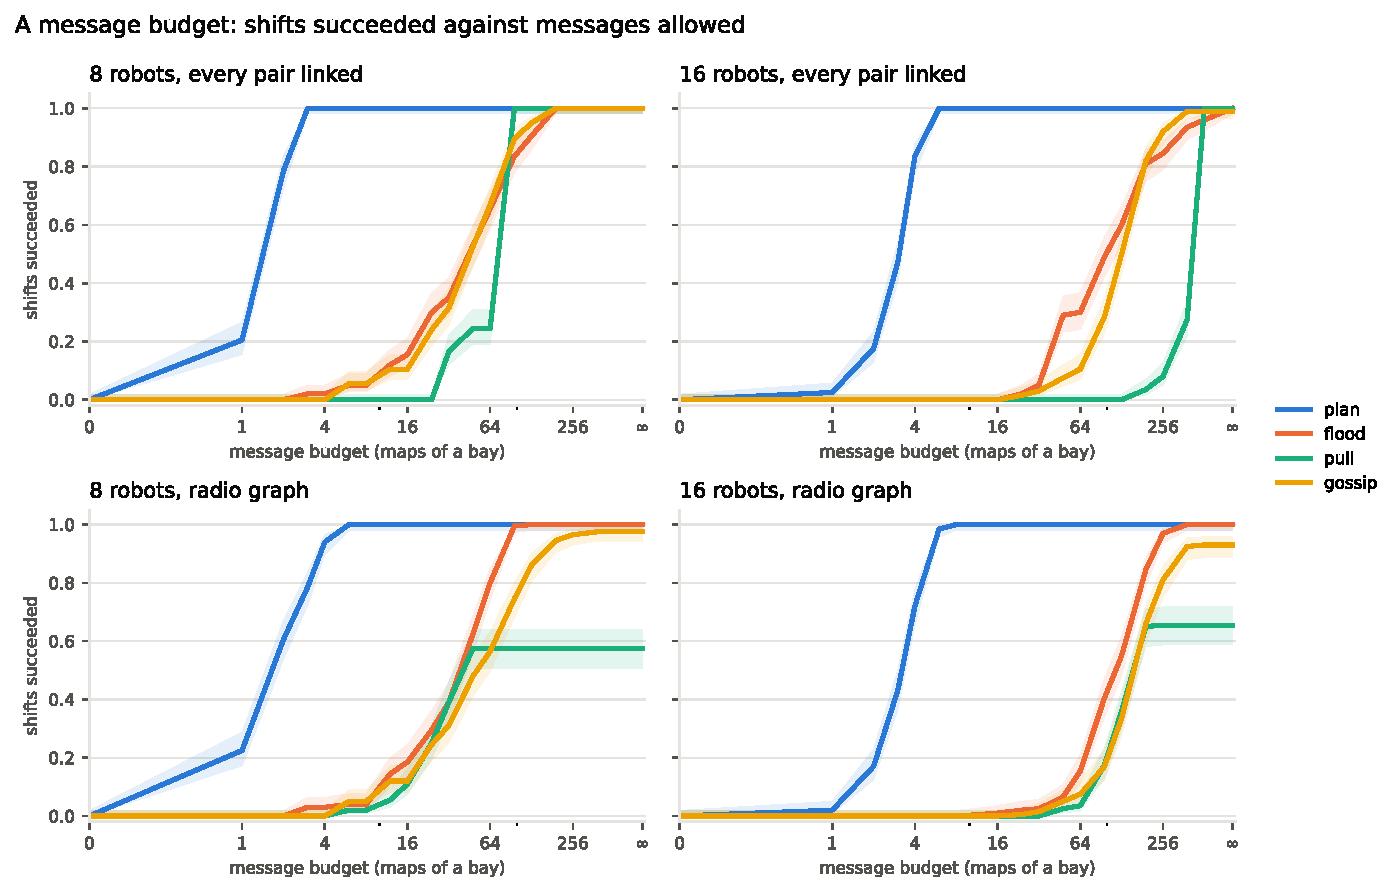
\includegraphics[width=\textwidth]{figures/regimes_budget.pdf}
\caption{Success against the message budget, with Wilson 95\% bands. The axis is
linear below 1 and logarithmic above; $\infty$ is no budget.}
\label{fig:budget}
\end{figure}

\begin{figure}[H]
\centering
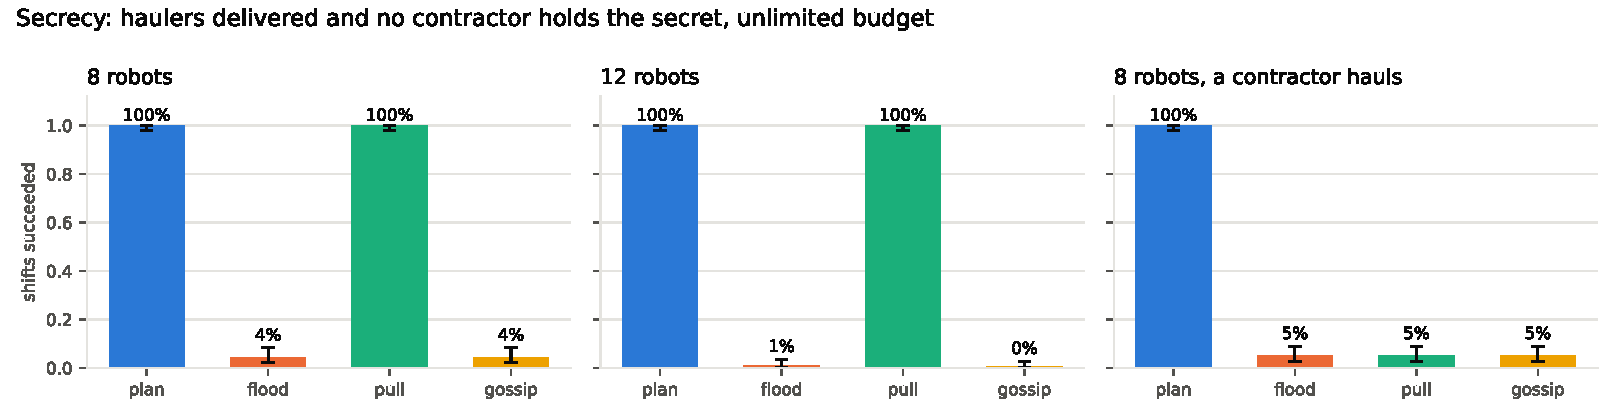
\includegraphics[width=\textwidth]{figures/regimes_secrecy.pdf}
\caption{Secrecy, without a budget. Flooding's and gossip's successes are the
instances in which nobody saw the staging; pull's are the same once the contractor
hauls.}
\label{fig:secrecy}
\end{figure}

\begin{figure}[H]
\centering
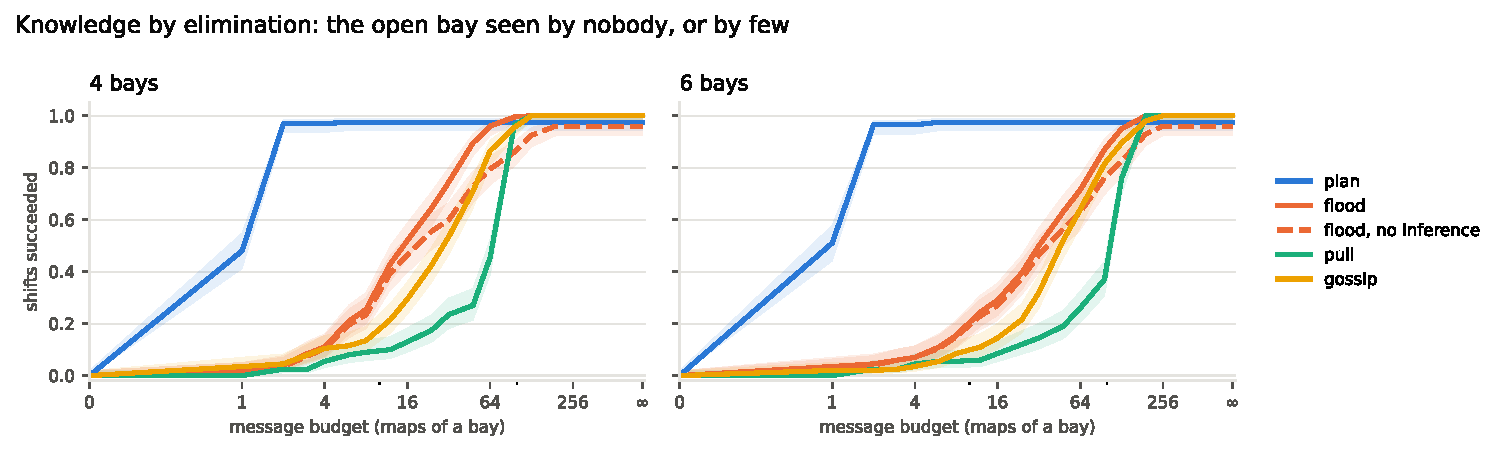
\includegraphics[width=\textwidth]{figures/regimes_elimination.pdf}
\caption{Elimination. The dashed curve is flooding with haulers that do not infer
a bay open from every other bay blocked.}
\label{fig:elim}
\end{figure}

\begin{figure}[H]
\centering
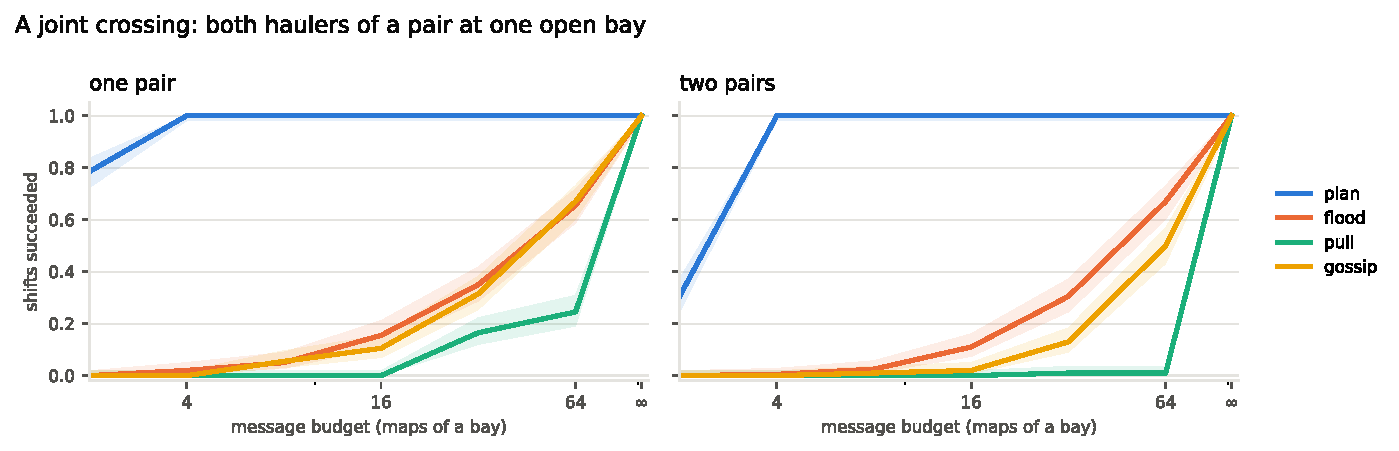
\includegraphics[width=0.95\textwidth]{figures/regimes_joint.pdf}
\caption{Joint crossing. No budget was tried between 64 and unlimited.}
\label{fig:joint}
\end{figure}

\begin{figure}[H]
\centering
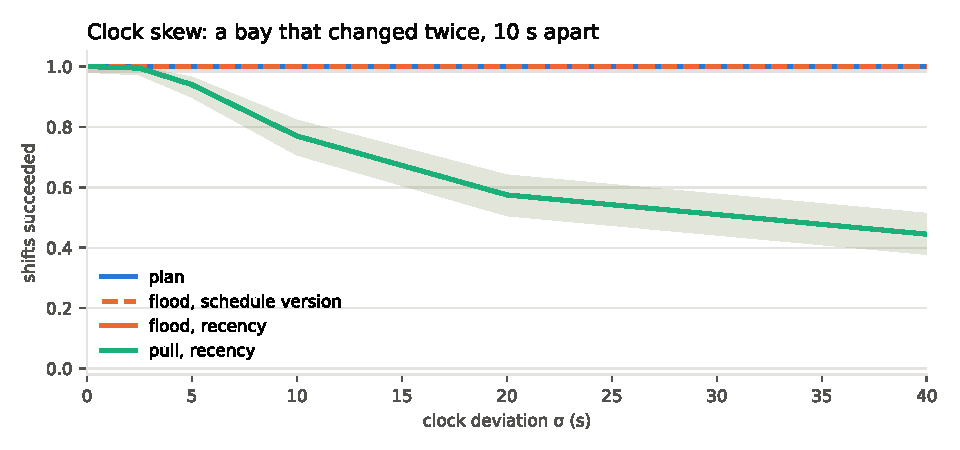
\includegraphics[width=0.7\textwidth]{figures/regimes_skew.pdf}
\caption{Clock skew, without a budget. The plan and flooding by version coincide
at 100\%; flooding and pull by recency coincide below them.}
\label{fig:skew}
\end{figure}

\paragraph{The plan's cost} The planner solved 2390 of the 2400 instances. The ten
it did not are elimination instances that ran out of the 120\,s limit, five with
four bays and five with six. The median solve time was 0.08\,s, the 95th percentile
2.9\,s and the largest 10.1\,s; among the cells without timeouts the slowest was
sixteen robots on a complete graph, median 1.7\,s. In 14 policies a robot sent a belief it held by inference
and not by observation, 18 messages in all. A protocol needs no solving at all, and
for the conditions of Proposition~\ref{prop:enough} that is the better trade.

\paragraph{An earlier pull} The first run of the study used a pull in which a
hauler stopped asking at the first bay it then believed open. It failed whenever a
staging nobody saw left the first bay open on every map, which flooding avoids by
choosing the freshest open reading. The pull reported here asks about every bay, the
stronger baseline; the first run's data are kept beside the second.

%  ======================================================================
\section{On the floor}
\label{sec:floor}

The stale-maps floor~\cite{ulises2026sm} has eight robots, three of which haul
($r_2$, $r_4$, $r_8$). The forklift clears $t_3$ and stages a load in $t_1$; two
robots see the clearing ($r_6$, $r_7$) and three the staging ($r_1$, $r_2$, $r_3$). On the secret floor $r_4$ is a
contractor's robot: it hauls, saw neither change, and must end the shift not
believing $t_1$ blocked. The goal is
\[
  \delivered(r_2) \wedge \delivered(r_4) \wedge \delivered(r_8) \wedge
  \neg\Bop{r_4}\blocked(t_1).
\]
Aletheia's policy is the one it finds without the secret: $r_6$ tells $r_2$ that
$t_3$ is open, $r_2$ tells $r_4$ and $r_8$, and each crosses $t_3$. No message is
about $t_1$. The protocols' sends were computed on this floor by the study's own
simulator and run by the mission in the same order, through the same relay the
plan's reports use, each moving a robot's living map. Before each run an analysis
predicted what it would do, and the mission checked the run against it.

\begin{table}[H]
\centering
\small
\begin{tabular}{@{}lrrl@{}}
\toprule
strategy & messages & delivered & contractor sent the secret \\
\midrule
flood, unlimited & 189 & 3 of 3 & yes, by $r_2$ \\
flood, stopped at 3 & 3 & 0 of 3 & no \\
pull & 126 & 3 of 3 & yes, by $r_1$ \\
\textbf{plan} & \textbf{3} & \textbf{3 of 3} & \textbf{no} \\
\bottomrule
\end{tabular}
\caption{The four runs in Gazebo. Pull's 126 are 63 requests and 63 replies. Every
run did what the analysis made before it said it would; in the plan's run, the
epistemic state and the robots' maps agreed on all 24 beliefs.}
\label{tab:floor}
\end{table}

\begin{figure}[H]
\centering
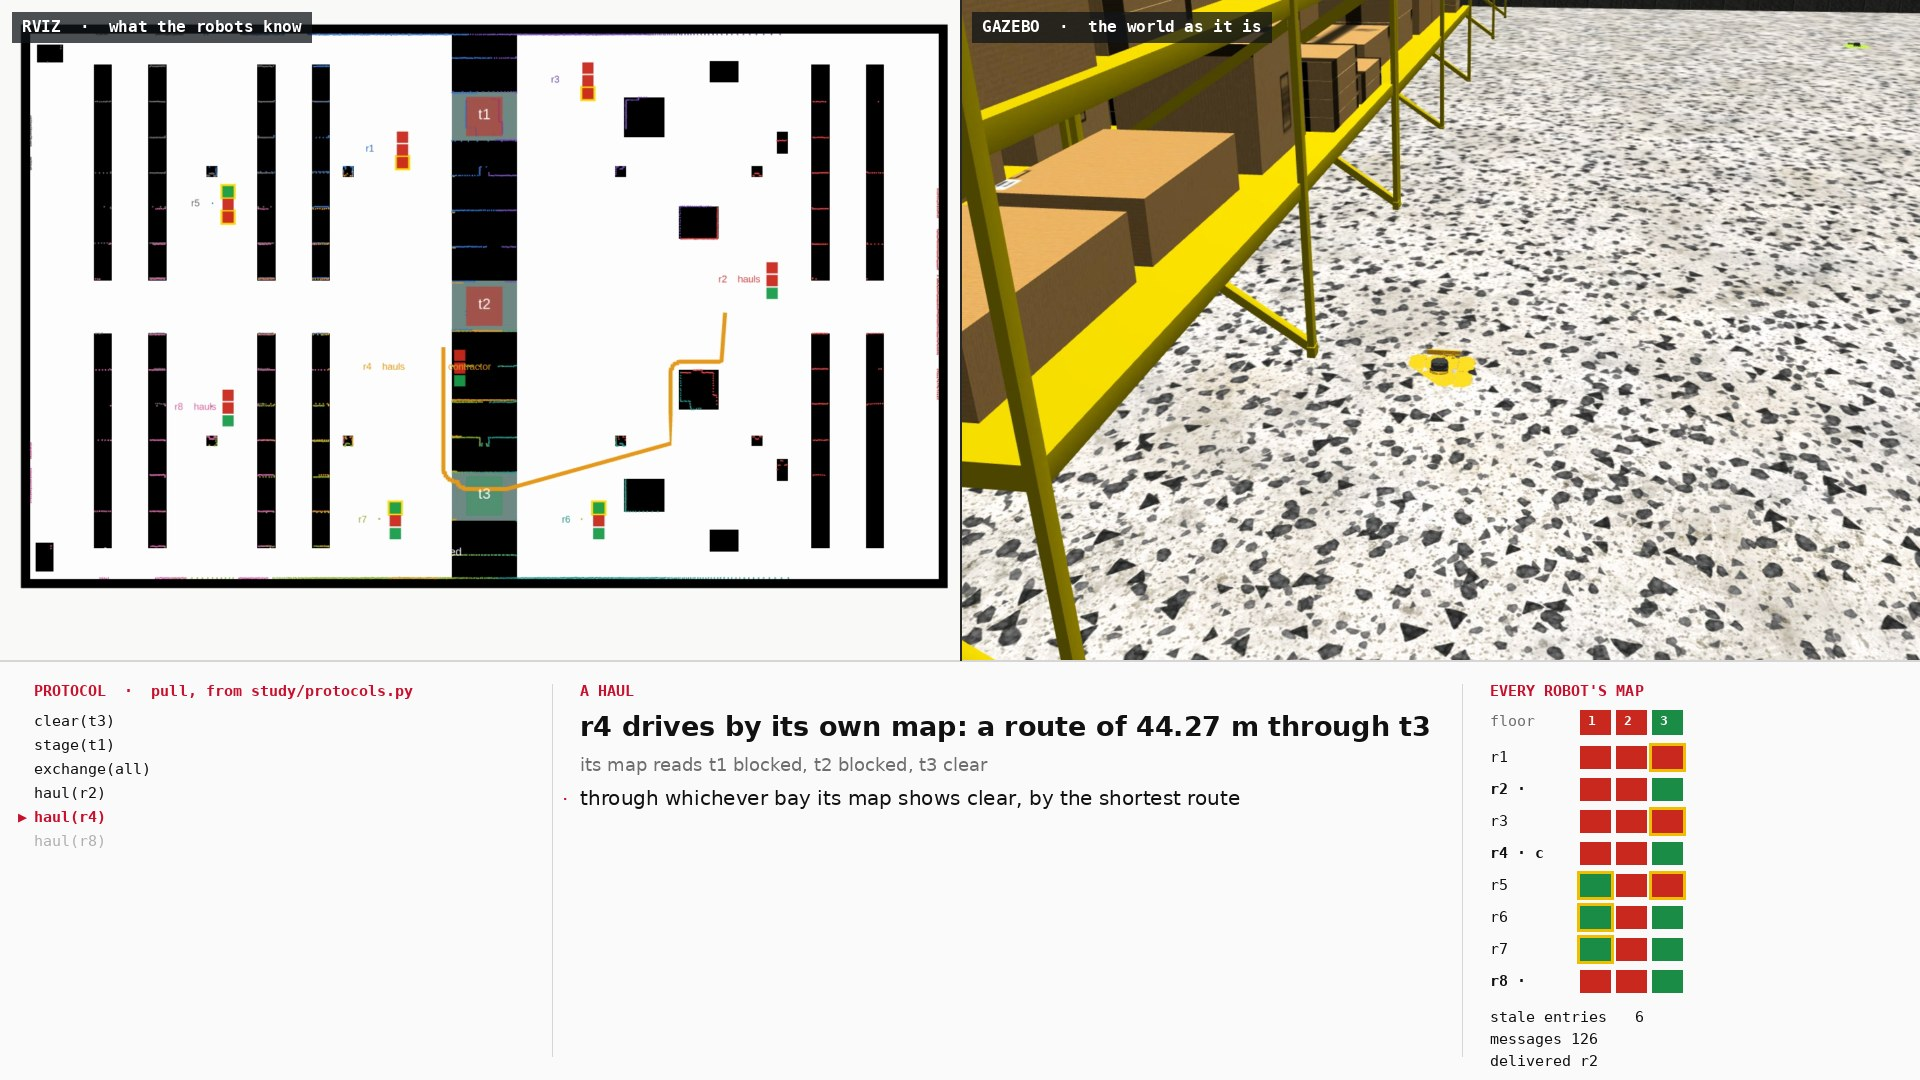
\includegraphics[width=\textwidth]{figures/regimes_secret_frame.jpg}
\caption{The pull run. $r_4$, the contractor (marked \emph{c}), drives through
$t_3$ with $t_1$ blocked on its map: it asked about $t_1$ and was told.}
\label{fig:frame}
\end{figure}

Flooding stopped at the plan's three messages delivered nothing: its first three
sends were $r_4$'s stale readings of the three bays, to $r_1$, which does not haul. The floor is one instance; the study is what
says how often each of these happens.

%  ======================================================================
\section{What this does not show}
\label{sec:limits}

\begin{itemize}[leftmargin=1.4em, itemsep=2pt]
  \item Protocols designed for a task. A protocol that knew the contractors and the
        secret, or which robots haul, could do what the plan does on these
        instances. The claim is that it would then encode the goal, which is what
        a planner takes as input.
  \item Lossy links, or messages that cost differently. Every message arrives,
        and every message costs one.
  \item Larger instances. The study stays at sixteen robots and six bays, where the
        planner solves within seconds; the stale-maps report found random fleets of
        64 robots unsolved within 600\,s.
  \item Shifts in which robots look again. Observation is transient here; a robot
        that re-read a bay would make stale readings rarer for every strategy.
\end{itemize}

\begin{thebibliography}{9}
\bibitem{bms1998} A.~Baltag, L.~S. Moss and S.~Solecki.
The logic of public announcements, common knowledge, and private suspicions.
\emph{Proceedings of TARK VII}, 43--56, 1998.
\bibitem{ba2011} T.~Bolander and M.~B. Andersen.
Epistemic planning for single- and multi-agent systems.
\emph{Journal of Applied Non-Classical Logics} 21(1):9--34, 2011.
\bibitem{fhmv1995} R.~Fagin, J.~Y. Halpern, Y.~Moses and M.~Y. Vardi.
\emph{Reasoning About Knowledge}. MIT Press, 1995.
\bibitem{lamport1978} L.~Lamport.
Time, clocks, and the ordering of events in a distributed system.
\emph{Communications of the ACM} 21(7):558--565, 1978.
\bibitem{ulises2026sm} H.~Ulises.
Maps that go stale: stale maps as false beliefs, and a received map as an update,
for a fleet of eight robots. Epistemic Robotics report, 2026.
\end{thebibliography}

\section*{Reproduction}

\begin{lstlisting}[language={}]
cd ros2_ws/src/stale_map_demo/study
python3 run_study.py --out /tmp/study --seeds 200 --workers 10   # 2400 instances, ~15 min
python3 analyze.py --csv /tmp/study/study.csv --out /tmp/study/analysis
cd ..
python3 tools/fleets.py --fleets secret flood flood3 pull         # the floor's predictions
ros2 launch stale_map_demo stale_maps_launch.py fleet:=secret      # also flood, flood3, pull
\end{lstlisting}

\end{document}
